%% Theorie.tex
%%
%\usepackage[ngerman]{babel}
%% ==============
\chapter{Algorithmen zur multivariaten Analyse}
\label{ch:algorithmen}
%% ==============

{\bibliographystyle{babalpha-fl}}	% german style

Multivariate Datenanalyse spielt in der experimentellen Hochenergiephysik eine entscheidente Rolle um die gr\"o\ss en gemessenen Datenmengen (big data) untersuchen und auswerten zu k\"onnen. Im folgenden Kapitel \ref{ch:algorithmen} werden zun\"achst einige Grundlagen der multivariaten Datenanalyse genannt, um sp\"ater genauer auf verschiedene Algorithmen und ihre Implementationen anhand kleinerer Beispiele einzugehen.

%% ===========================
\section{Grundlagen zur multivariaten Datenanalyse}
\label{ch:Theorie:sec:Algorithmen}
%% ===========================

Datenanalyse bezeichnet statistische Verfahren, mit deren Hilfe aus numerischen Daten Informationen gewonnen werden sollen.
Bei multivariaten Analysemethoden werden mehrere Eingabegr\"o\ss en zugleich statistisch untersucht, dadurch ist eine Berechnung sehr aufw\"andig und somit manuell nicht zu bewerkstelligen. Mithilfe der zunehmenden Rechenleistung aktueller Computer ist dies jedoch m\"oglich und wird in vielen Bereichen immer wichtiger, beispielsweise im Finanzwesen, bei Studien zum Konsumverhalten, oder der Sprach-, Schrift- und Bilderkennung.
Die dazu verwendeten Algorithmen bezeichnet man auch als maschinelles Lernen (machine learning), da mit ihrer hilfe versucht wird, aus den Daten zu lernen und Vorhersagen zu treffen. Man unterscheidet zwischen Regression (regression), bei der eine kontinuirliche Ausgangsgr\"o\ss e gesucht wird und Klassifizierung (classification), bei der eine diskrete Antwort gesucht wird.\cite{SWB-455193959} Im Fall der \ttH-Analyse werden Regre\ss ionsmodelle verwendet um physikalische Gr\"o\ss en wie beispielsweise die Higgsbosonmasse zu rekonstruieren. Bei der Klassifizierung wird dagegen versucht, ein Ereignis einer Klasse zuzuordnen, also entweder Signal (englisch signal) oder Untergrund (englisch background). Im Folgenden werden ausschlie\ss lich Klassifizierungsprobleme behandelt.

Es existieren verschiedene Ans\"atze zur Klassifizierung. Einer dieser Ans\"atze ist das \"uberwachte Lernen (supervised learning). Beispiele sind die St\"utzvektormethode, wobei jedoch die englische Bezeichnung support vector machine (SVM) gebr\"auchlich ist, Random Forest (RF), was Zuf\"alliger Wald bedeutet und mehrere zuf\"allig erstellte Entscheidungsb\"aume (Abschnitt \ref{ch:Algorithmen:subsec:Entscheidungsbaum} bezeichnet, oder Neuronale Netze. Ein weiteres Beispiel sind verst\"arkte Entscheidungsb\"aume (Boosted Decision Trees (BDTs)). Da hiervon verschiedene Implementationen im Kapitel \ref{ch:vergleich} untersucht und getestet werden sollen, werden sie im folgenden Abschnitt \ref{ch:Algorithmen:sec:BDT} genauer beschrieben.

%% ===========================
\section{Boosted Decision Trees (BDTs)}
\label{ch:Algorithmen:sec:BDT}
%% ===========================

Boosted Decision Trees sind eine h\"aufig genutze Methode der multivariaten Datenanalyse. Im folgenden werden sie anhand eines einfachen Beispiels erkl\"art. Bei diesem handelt es sich um zwei zweidimensionale Gau\ss kurven die sich \"uberlappen. Eine stellt das Signal dar, die andere dient als Hintergrund. In den Abbildungen \ref{fig:2dgauss_histX} und \ref{fig:2dgauss_histY} sind die Verteilungen der trennenden Variablen X und Y dargestellt.\\
Die folgenden Abschnitte sind gr\"o\ss tenteils an \cite{SWB-307748006} angelehnt.

%% ===========================
\subsection{Entscheidungsb\"aume}
\label{ch:Algorithmen:subsec:Entscheidungsbaum}
%% ===========================

Entscheidungsb\"aume unterteilen den Bereich des zu klassifizierenden Objektes anhand gerader Schnitte auf dessen Eigenschaften (Variablen) in mehrere Sequenzen. Wieviele dieser Sequenzen ab dem Wurzelknoten erstellt werden, wird durch die Tiefe (depth) des Baumes angegeben. Man unterscheidet zwischen zwei Arten, bin\"aren B\"aumen mit diskreten R\"uckgabewerten zur Unterscheidung mehrerer Klassen (classification trees), zum Beispiel Signal und Untergrund, sowie denjenigen mit kontinuierlicher Antwort (regression trees). \cite{SWB-455193959} Eine h\"aufige Implementation von Entscheidungsb\"aumen ist CART (classification and regression trees), so implementierte B\"aume eignen sich sowohl f\"ur Klassifikationen als auch f\"ur Regressionen.\\
In Abbildung \ref{fig:DecicionTree} ist ein Beispiel eines Baumes mit der Tiefe zwei zu sehen. An jedem Knoten werden die Objekte aufgrund ihrer Eigenschaften und Kriterien in Signal und Untergrund unterteilt. Im Wurzelknoten ist der erste diskriminierende Schnitt angegeben. Alle Objekte mit einem Y-Wert gr\"o\ss er als 0.33 werden als eher Hintergrundartig eingestuft. In der n\"achsten Stufe des Baumes werden f\"ur jede der beiden zuvor getrennten Mengen Schnitte auf den X-Wert angewendet. In Abbildung \ref{fig:depht2} ist die Ausgabe (output) dieses Baumes abgebildet, das heist jedem Punkt wird entsprechend seiner X- und Y-Koordinaten ein Wert zugeordnet, der angibt, ob der Punkt eher als Signal oder als Untergrund klassifiziert wurde. H\"ohere Werte (rote F\"arbung) werden f\"ur signalartige Punkte verwendet, niedrigere (blaue F\"arbung) f\"ur hintergrundartige. Man erkennt deutlich die verschiedenen Schnitte des Baumes.\\
%\begin{figure}[hhh]
% \begin{center}
%  \begin{minipage}[b]{0.5\textwidth}  
%   \includegraphics[width=\textwidth]{graphics/tree.pdf}
%   \centering (a)
%  \end{minipage}%
%  \begin{minipage}[b]{0.5\textwidth}
%   \includegraphics[width=\textwidth]{graphics/tree_depht2.pdf}
%   \centering (b)
%  \end{minipage}
%   \parbox[b]{12cm}{
%     \caption[Entscheidungsbaumes der Tiefe 2]
%             {\label{fig:DecicionTree} \it schematische Abbildung eines Entscheidungsbaumes der Tiefe 2. X und Y sind die Variablen anhand denen durch cuts (Zahlen nach den Variablen) zwischen Untergrund und Signal unterschieden werden soll.\\Erstellt mit TMVA}
%   }
% \end{center}
%\end{figure}

\begin{figure}[hhh]
\centering     %%% not \center
\subfigure[Entscheidungsbaum der Tiefe 2]{\label{fig:DecicionTree}\includegraphics[width=0.49\textwidth]{graphics/tree.pdf}}
\subfigure[Klassifiezierung des Baumes]{\label{fig:depht2}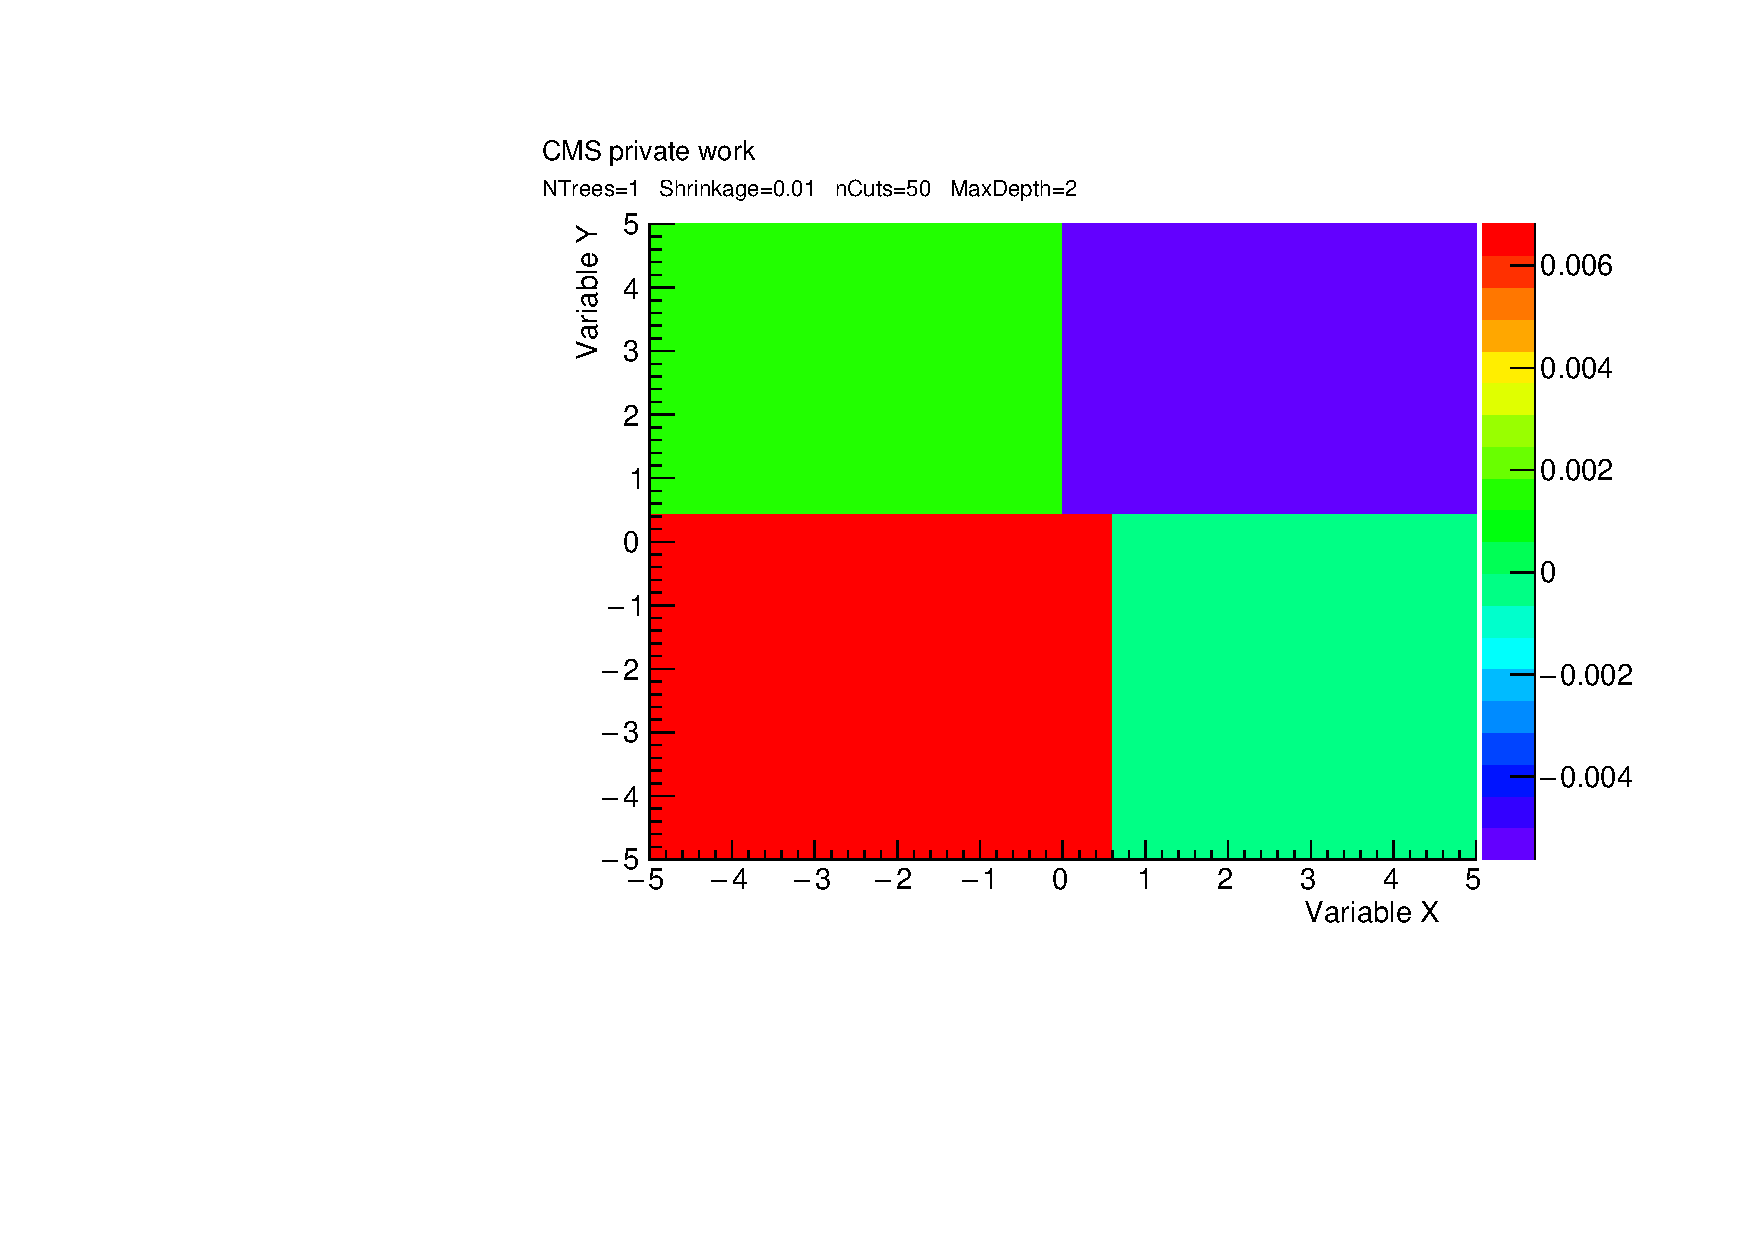
\includegraphics[width=0.49\textwidth]{graphics/tree_depht2_1.pdf}}
\caption{\it Links ist eine schematische Abbildung eines Entscheidungsbaumes der Tiefe 2 abgebildet. X und Y sind die Variablen anhand denen durch Schnitte (Zahlen nach den Variablen) zwischen Untergrund und Signal unterschieden werden soll. Die rechte Graphik zeigt die Klassifizierung die mithilfe des Baumes erstellt wurde.}
\end{figure}


Die Trennung ist allerdings noch sehr grob, selbst wenn man die Tiefe des Baumes deutlich erh\"oht, wie in \ref{fig:tree_100} mit der Tiefe 100 zu sehen, wird diese nicht deutlich besser. Dies ist beispielsweise m\"oglich indem man mehrere Entscheidungsb\"aume so miteinander verkn\"upft, dass sie zusammen eine starke Klassifizierung erm\"oglichen. Eine dieser Methoden ist das Verst\"arken von Entscheidungsb\"aumen (Boosting).




%BDTs vereinen durch Boosting und Bagging (aus dem Englischen von bootstrap aggregation abgeleitet) mehrere Entscheidungsb\"aume zu einem starken Kla\ss ifikator.

%% ===========================
\subsection{Verst\"arken von Entscheidungsb\"aumen (Boosting)}
\label{ch:Algorithmen:subsec:Boosting}
%% ===========================

Durch Boosting soll die G\"ute der Klassifizierung eines einzelnen Baumes erh\"oht werden. Dazu werden mehrere B\"aume hintereinander trainiert. Damit diese sich voneinander unterscheiden, wird nach jedem Training eine Umgewichtung der Ereignisse vorgenommen. Zun\"achst haben alle Ereignisse die gleiche Gewichtung. (In der \ttH-Analyse haben Ereignisse schon zuvor Gewichte, diese sind jedoch physikalisch motiviert.) Danach werden falsch klassifizierte Ereignisse st\"arker gewichtet und ein neuer Baum trainiert. Dies wird je nach geforderter Anzahl an Entscheidungsb\"aumen wiederholt.\\
In Abbildung \ref{fig:boosting} sind zum Vergleich die R\"uckgabewerte von einem einzelnen Entscheidungsbaum der Tiefe 100 (\ref{fig:tree_depht100}) sowie diejenigen von BDTs mit zwei (\ref{fig:BDT_nTree2}), zehn (\ref{fig:BDT_nTree10}) und hundert (\ref{fig:BDT_nTree100}) Boosting-Schritten gezeigt. Man erkennt, dass bei diesem einfachen Beispiel die Ausgabe der geboosteten Entscheidungsb\"aume schon ab zehn Einzelb\"aumen deutlich glatter wird und eine st\"arkere Unterscheidung vornehmen.

\begin{figure}[hhh]
\centering     %%% not \center
\subfigure[Klassifikation eines Baumes der Tiefe 100]{\label{fig:tree_depht100}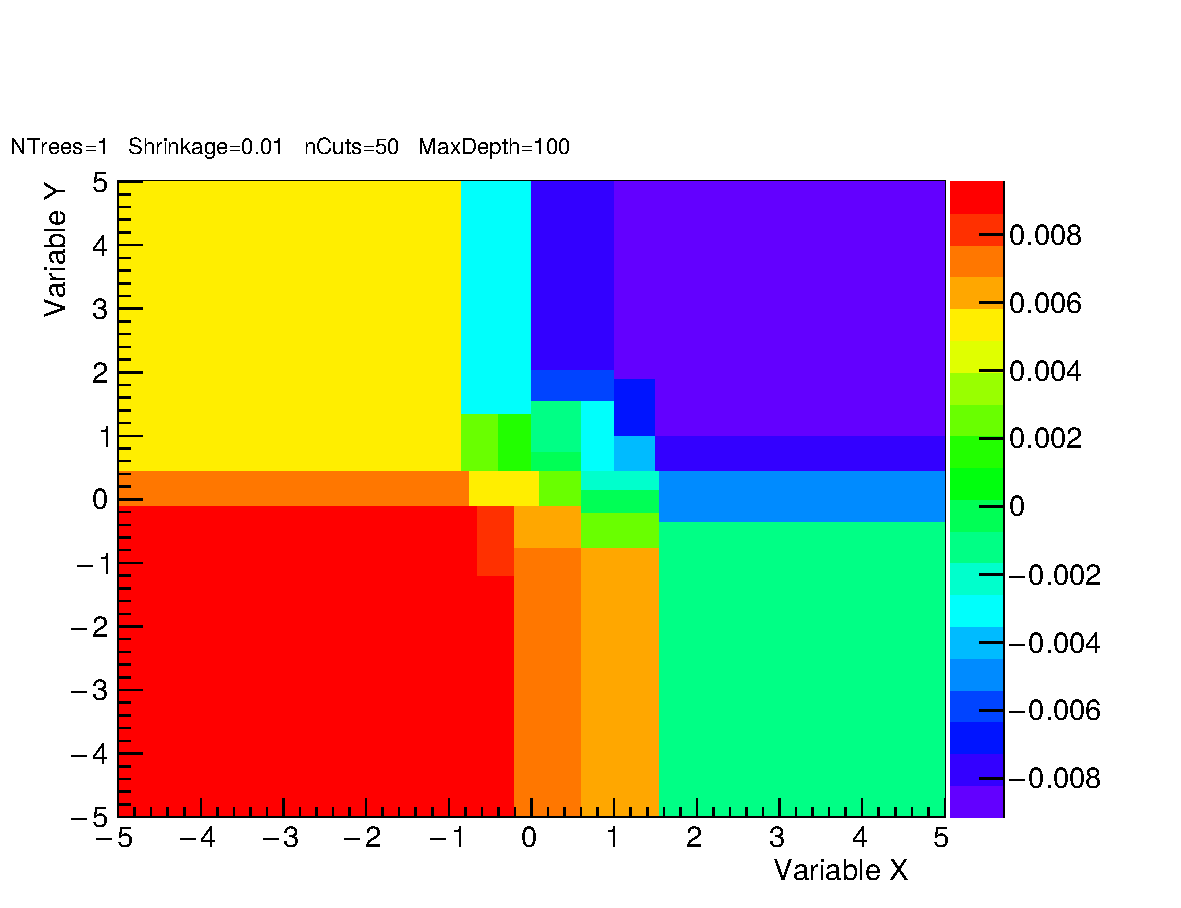
\includegraphics[width=0.49\textwidth]{graphics/tree_depht100.pdf}}
\subfigure[BDT Klassifikation mit 2 Trees]{\label{fig:BDT_nTree2}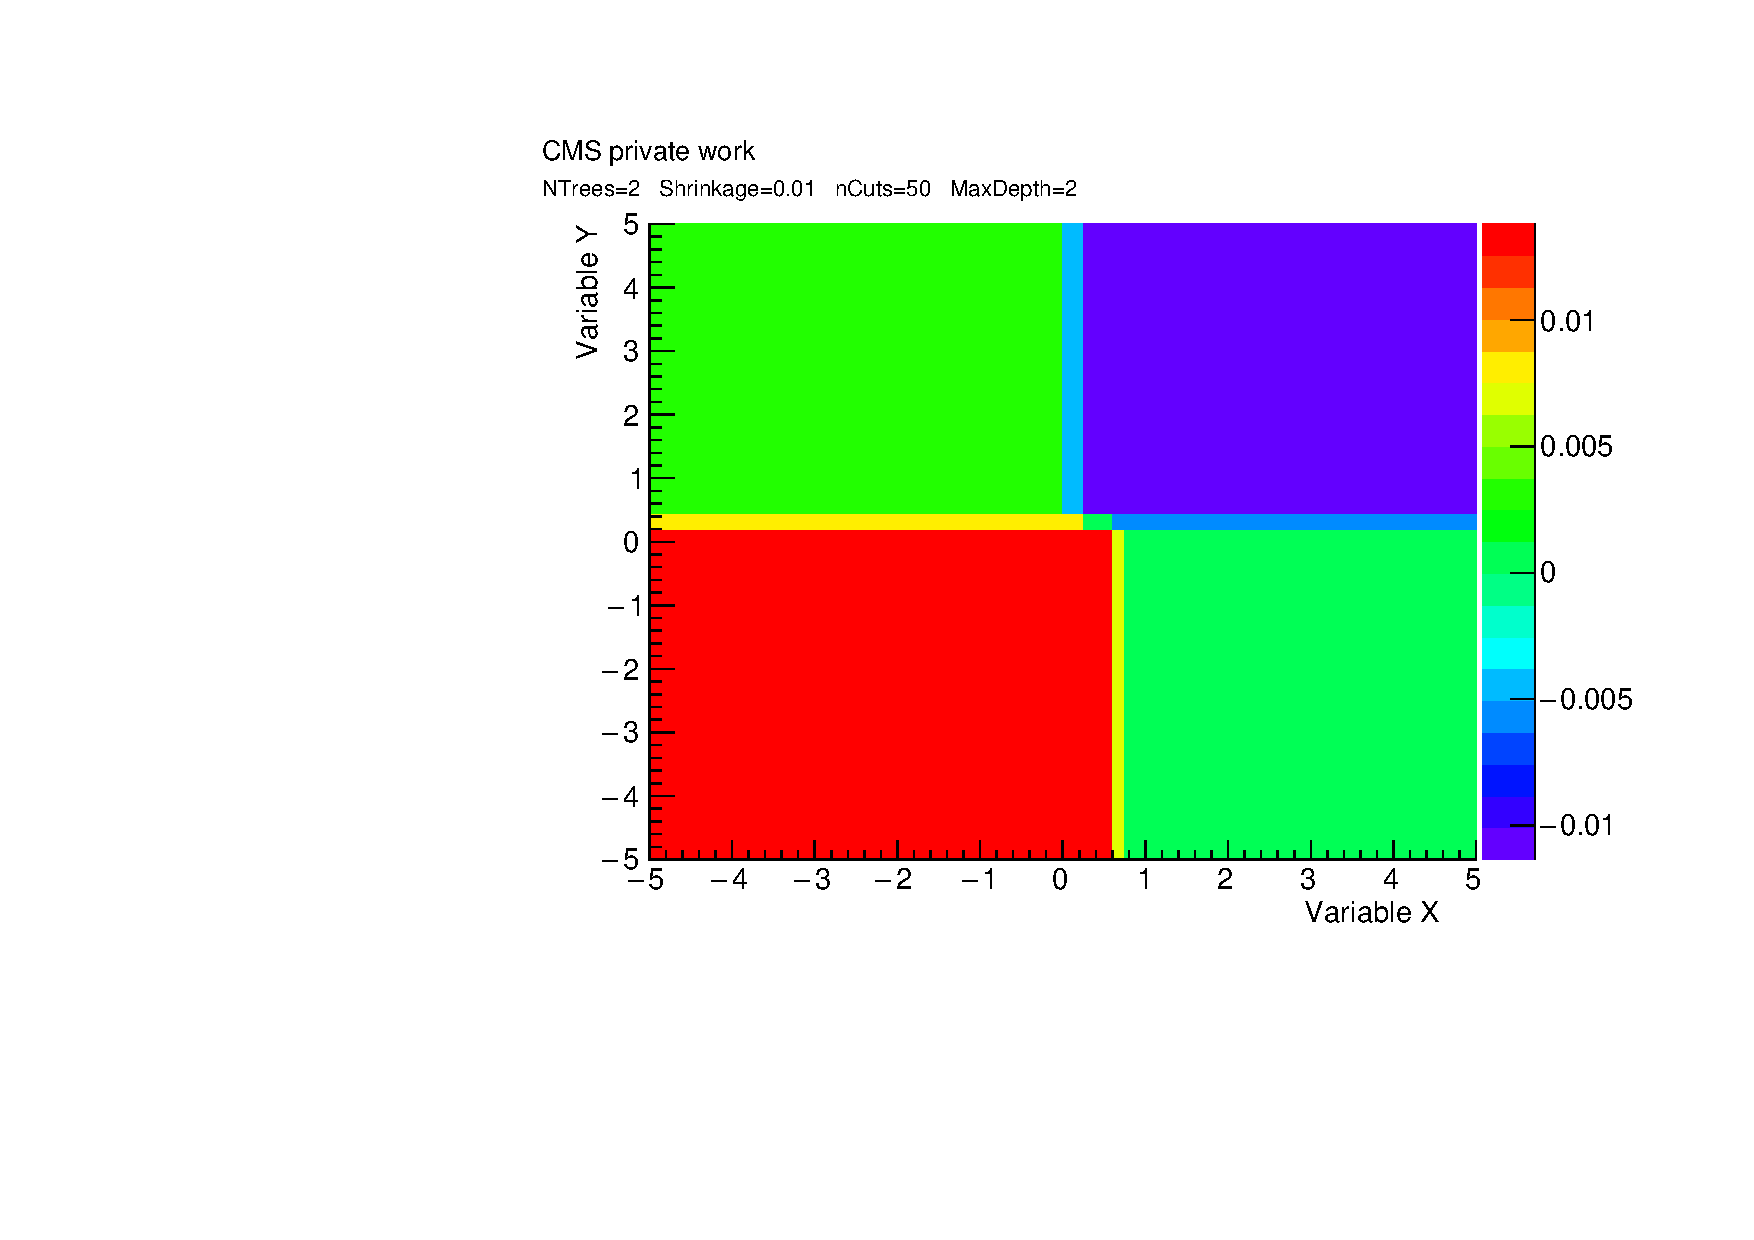
\includegraphics[width=0.49\textwidth]{graphics/tree_depht2_2.pdf}}
\subfigure[BDT Klassifikation mit 10 Trees]{\label{fig:BDT_nTree10}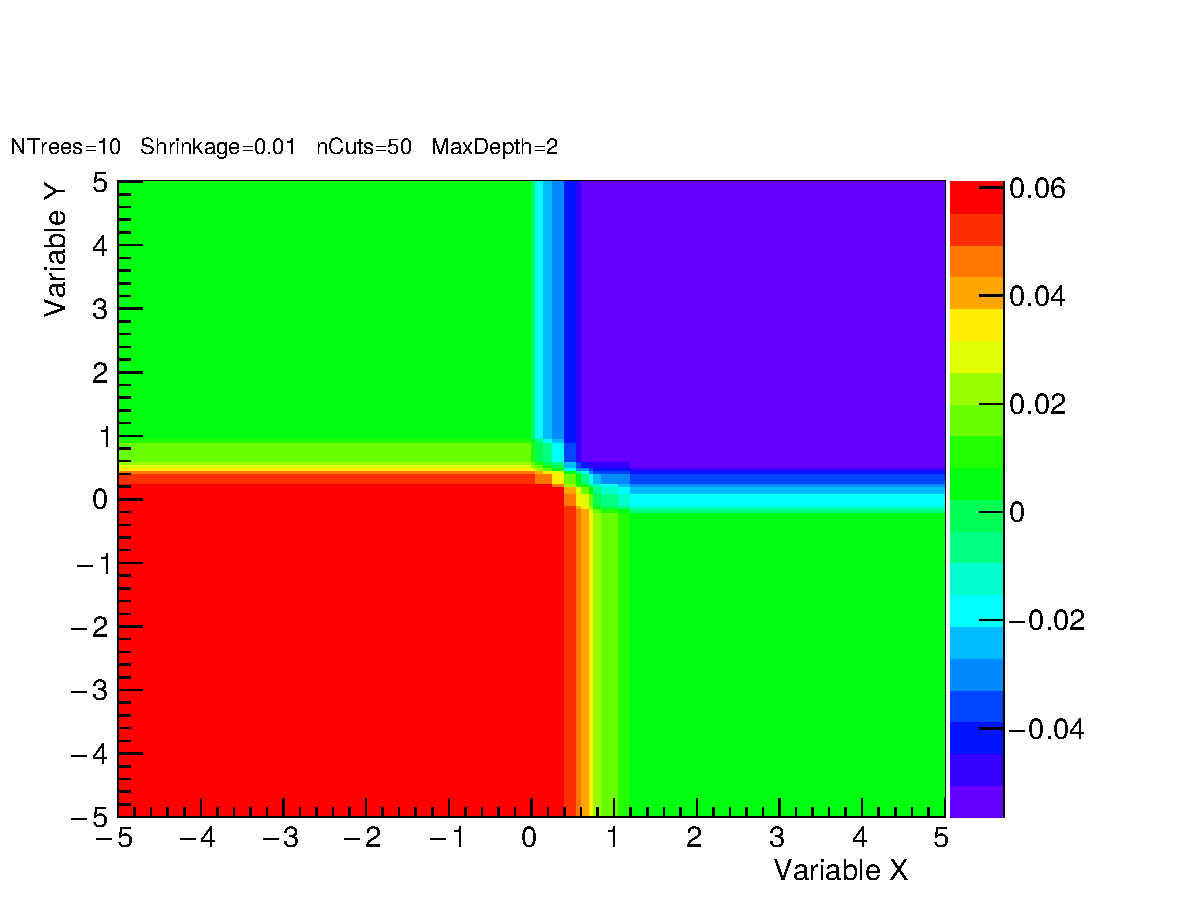
\includegraphics[width=0.49\textwidth]{graphics/tree_depht2_3.pdf}}
\subfigure[BDT Klassifikation mit 100 Trees]{\label{fig:BDT_nTree100}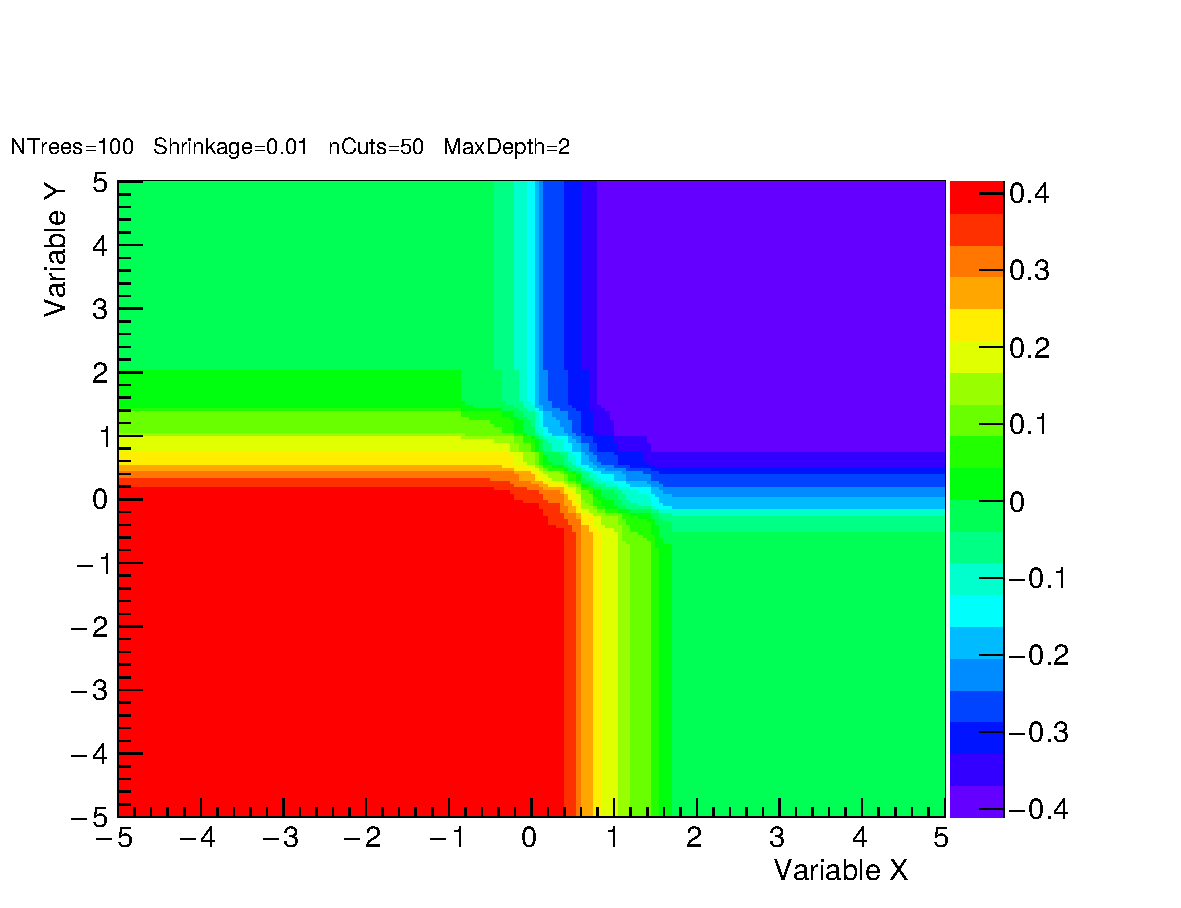
\includegraphics[width=0.49\textwidth]{graphics/tree_depht2_4.pdf}}
\caption{\it (a) zeigt die Klassifikation, die mit einem einzelnen Entscheidungsbaum der Tiefe 100 erreicht wird. In den \"ubrigen Graphiken ist jeweils die Klassifikation eines BDT mit (b) 2 B\"aumen, (c) 10 B\"aumen und (d) 100 B\"aumen zu sehen.}
\label{fig:boosting}
\end{figure}

Die einfachste Methode ist, das Gewicht jedes falsch klassifizierten Ereignisses auf die gleiche Weise anzupassen. Eine weitere Verbesserung l\"asst sich erziehlen, indem man eine Ausgleichsfunktion (loss function) einf\"uhrt. Diese ordnet jedem Ereignis ausgehend vom aktuellen BDT-Output einen Wert zu, der bei richtiger Klassifikation minimal ist. Dadurch ist es m\"oglich, die Gewichte so anzupassen, dass die Ausgleichsfunktion minimiert wird.

%% ===========================
\section{Verwendete Algorithmen zur multivariaten Analyse}
\label{ch:Algorithmen:subsec:Implementationen}
%% ===========================

%% ===========================
\subsection{Toolkit for Multivariate Analysis in ROOT (TMVA)}
\label{ch:Algorithmen:subsec:TMVA}
%% ===========================

%% ===========================
\subsection{scikit-learn -- machine learning in python}
\label{ch:Algorithmen:subsec:sklearn}
%% ===========================

%% ===========================
\subsection{Extreme Gradient Boosting (XGBoost)}
\label{ch:Algorithmen:subsec:XGB}
%% ===========================
